% CHAPTER 4: SYSTEM ARCHITECTURE DESIGN
% ======================================================================
{\fontsize{18}{22}\selectfont\textbf{4 System Architecture Design}}\par

\vspace{3mm}

\subhead{4.1 Five-Layer Architecture Overview}

This platform adopts a five-layer architecture with high cohesion and low coupling, implementing one-way dependencies between layers: data is transmitted downwards via RESTful APIs, and long-lived connections are established upwards via WebSockets to proactively push events. This meets the requirements of banking systems for ``modularity,'' ``testability,'' and ``independent scalability.''

The five-layer structure described above is shown in the diagram below.

\begin{figure}[H]
\centering
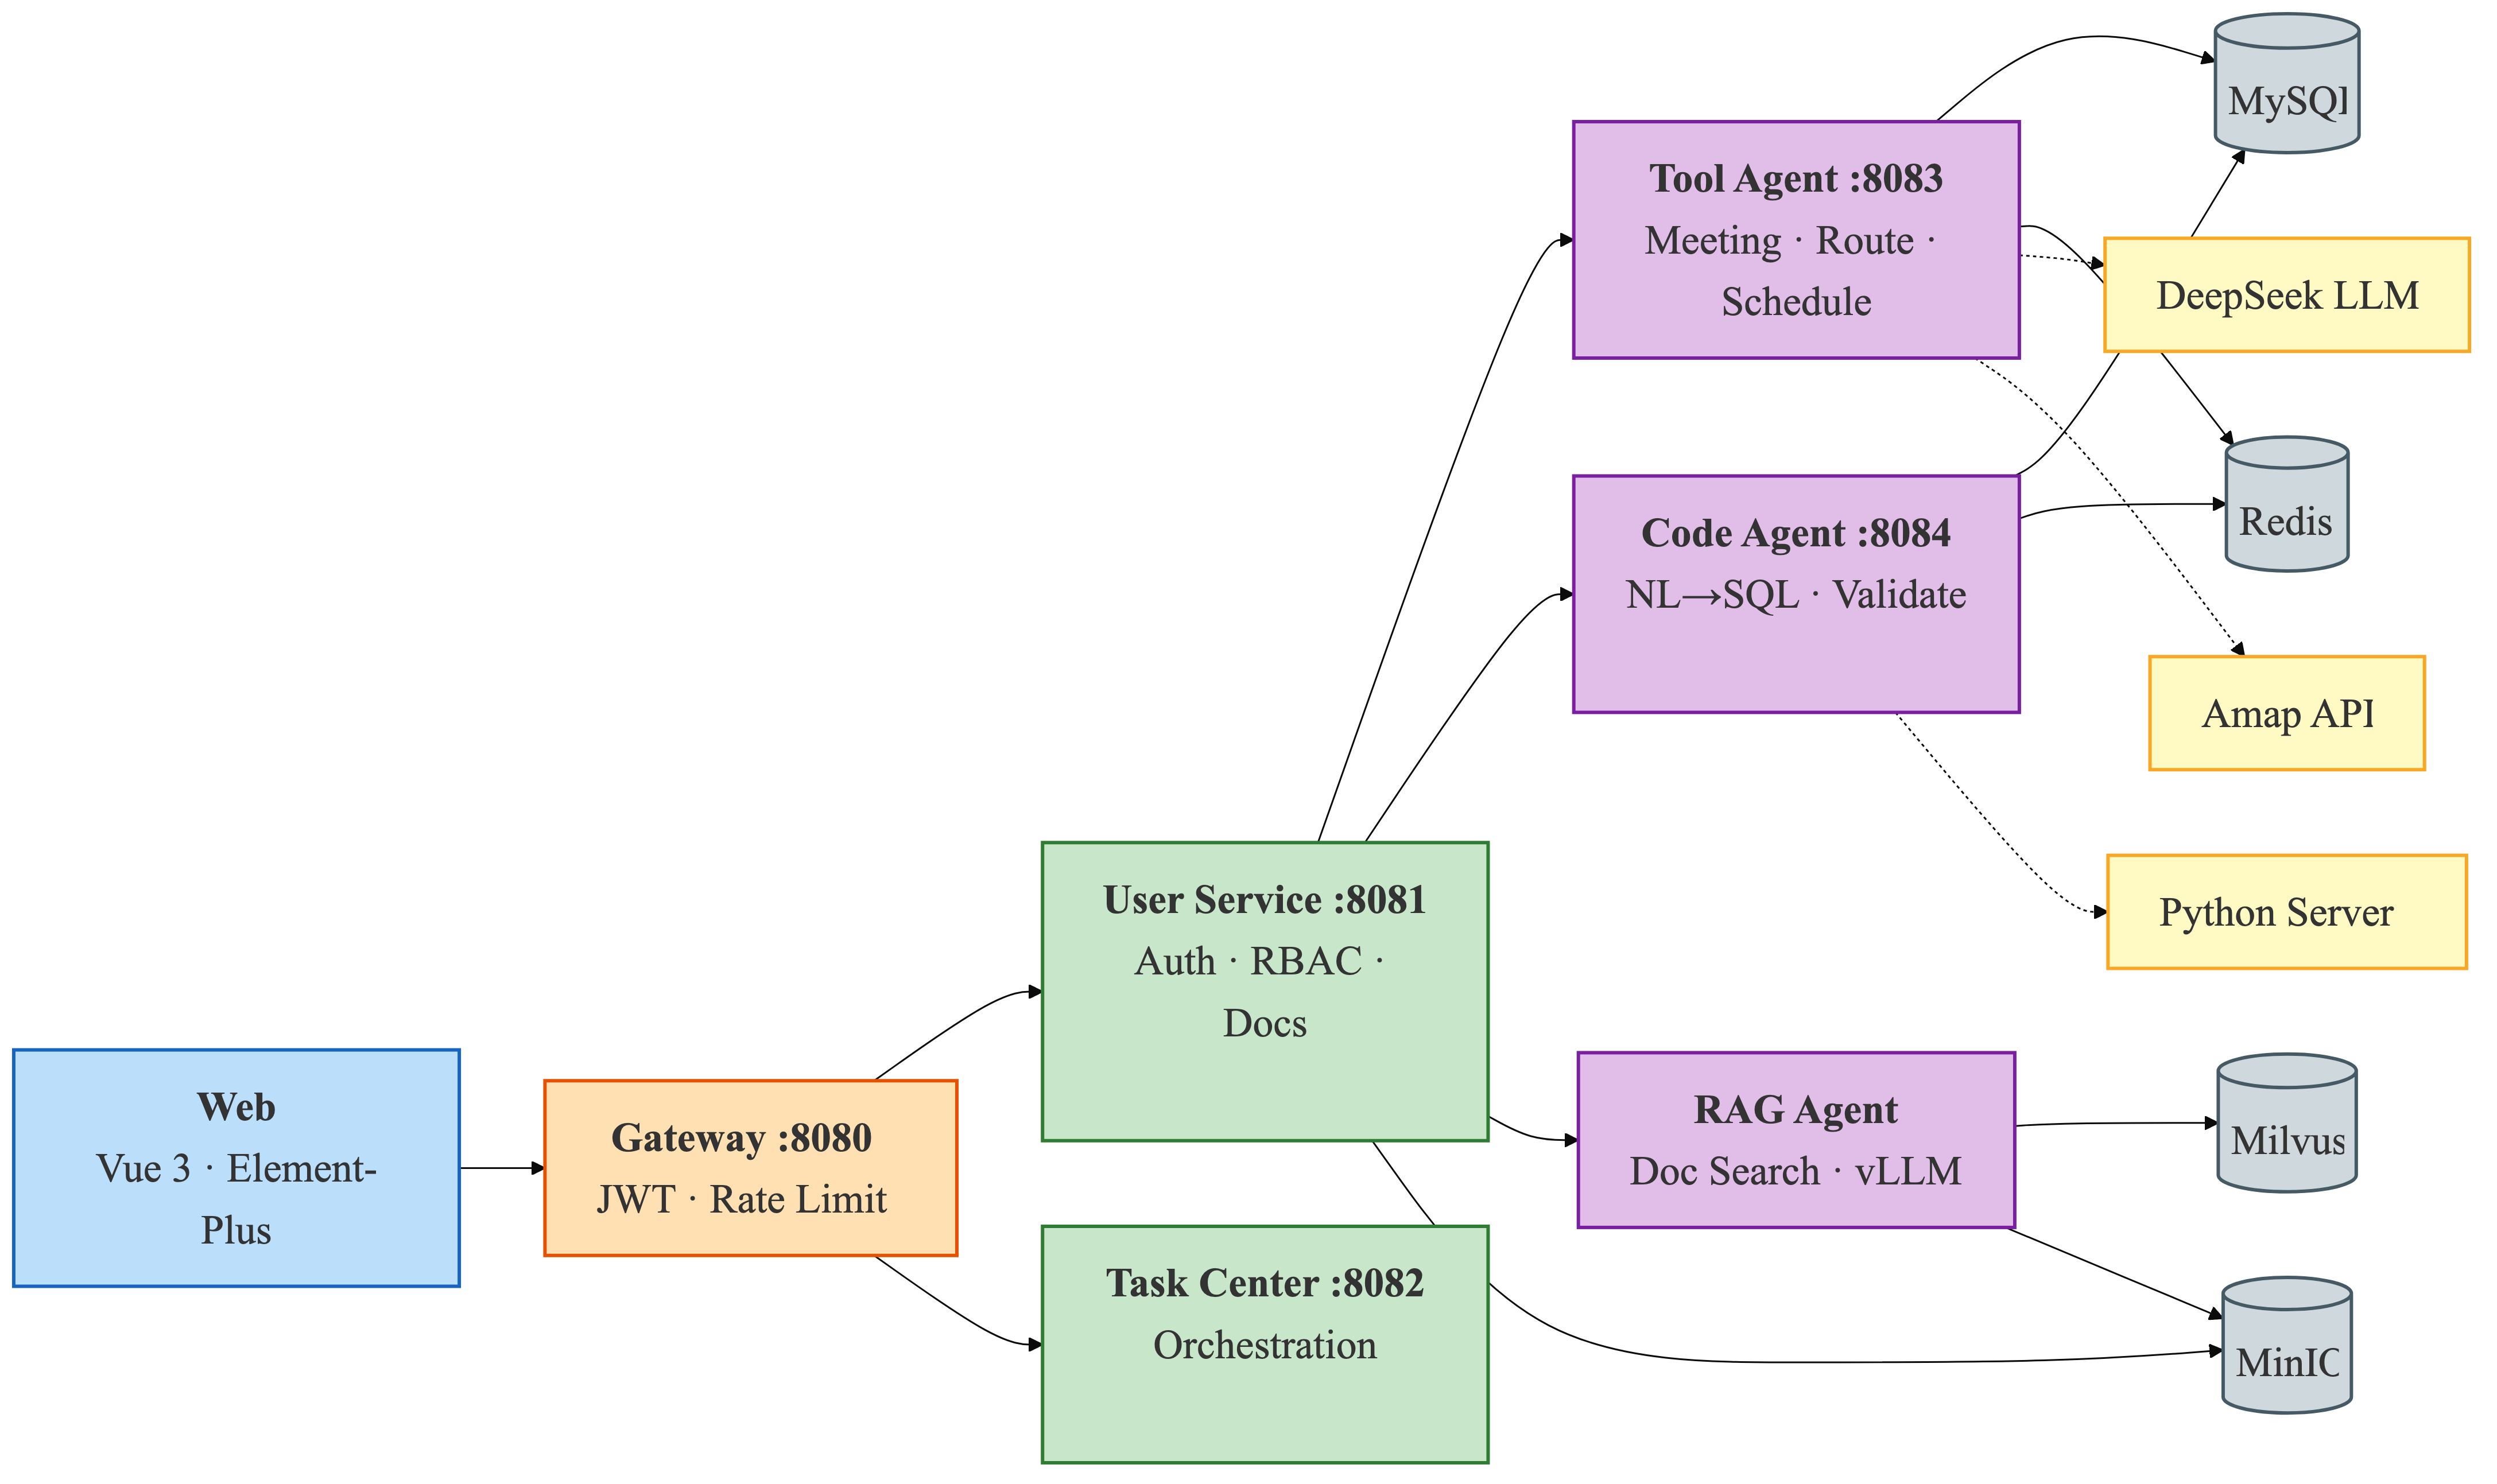
\includegraphics[width=0.92\textwidth]{figures/fig02_five_layer_arch.png}
\caption{Five-Layer Logical System Architecture --- Web, Gateway, Business Service, AI Service, and Data Layers}
\label{fig:five-layer}
\end{figure}

The five layers, from top to bottom, are as follows:

Layer 1 -- Web Presentation Layer. This is the front end of the architecture, using Vue 3 SPA, responsible for user interaction, result display (tables/maps/charts), and real-time progress push notifications. It supports Simplified Chinese, Traditional Chinese, and English language switching.

Layer 2 -- the gateway layer. As the system's sole entry point, the gateway layer is responsible for request routing and identity verification. Confidentiality is paramount in banking systems; requests not on the whitelist must be verified using JWT. Upon successful verification, the user's identity and permissions information are extracted and passed to downstream services.

Layer 3 -- Business Service Layer. This layer includes user services and a task center. User services handle registration and login, JWT issuance, and role-based access control; the task center handles cross-agent request scheduling and status management.

Layer 4 -- AI Service Layer. The AI layer deploys three dedicated agents: the Code Agent handles code generation and security verification before SQL execution; the Tool Agent handles enterprise tool requests, using a large model for intent recognition and parameter extraction; and the RAG Agent combines vector retrieval and generation models to provide policy Q\&A with cited sources.

The fifth layer -- the data layer. This is the lowest layer of the platform. We adhere to the principle of adapting to local conditions, using MySQL as the single data source to persistently store user, permission, organizational structure, document, and meeting room data; Redis is responsible for caching hot data (such as table structure metadata and schedule conflict detection); Milvus 2.3+ is deployed independently to handle document vectorization storage and semantic retrieval, providing the RAG Agent with similarity search capabilities.

The request lifecycle shown in Figure \ref{fig:data-flow} varies significantly depending on the ingress type. We assume all external traffic first flows into the gateway layer. JWT authentication and rate limiting policies are strictly implemented upfront---the legitimacy of the request and the access rate are determined before routing decisions are made (otherwise, network security issues could easily arise). Only traffic that passes through this filtering layer is allowed to proceed downstream.

\begin{figure}[H]
\centering
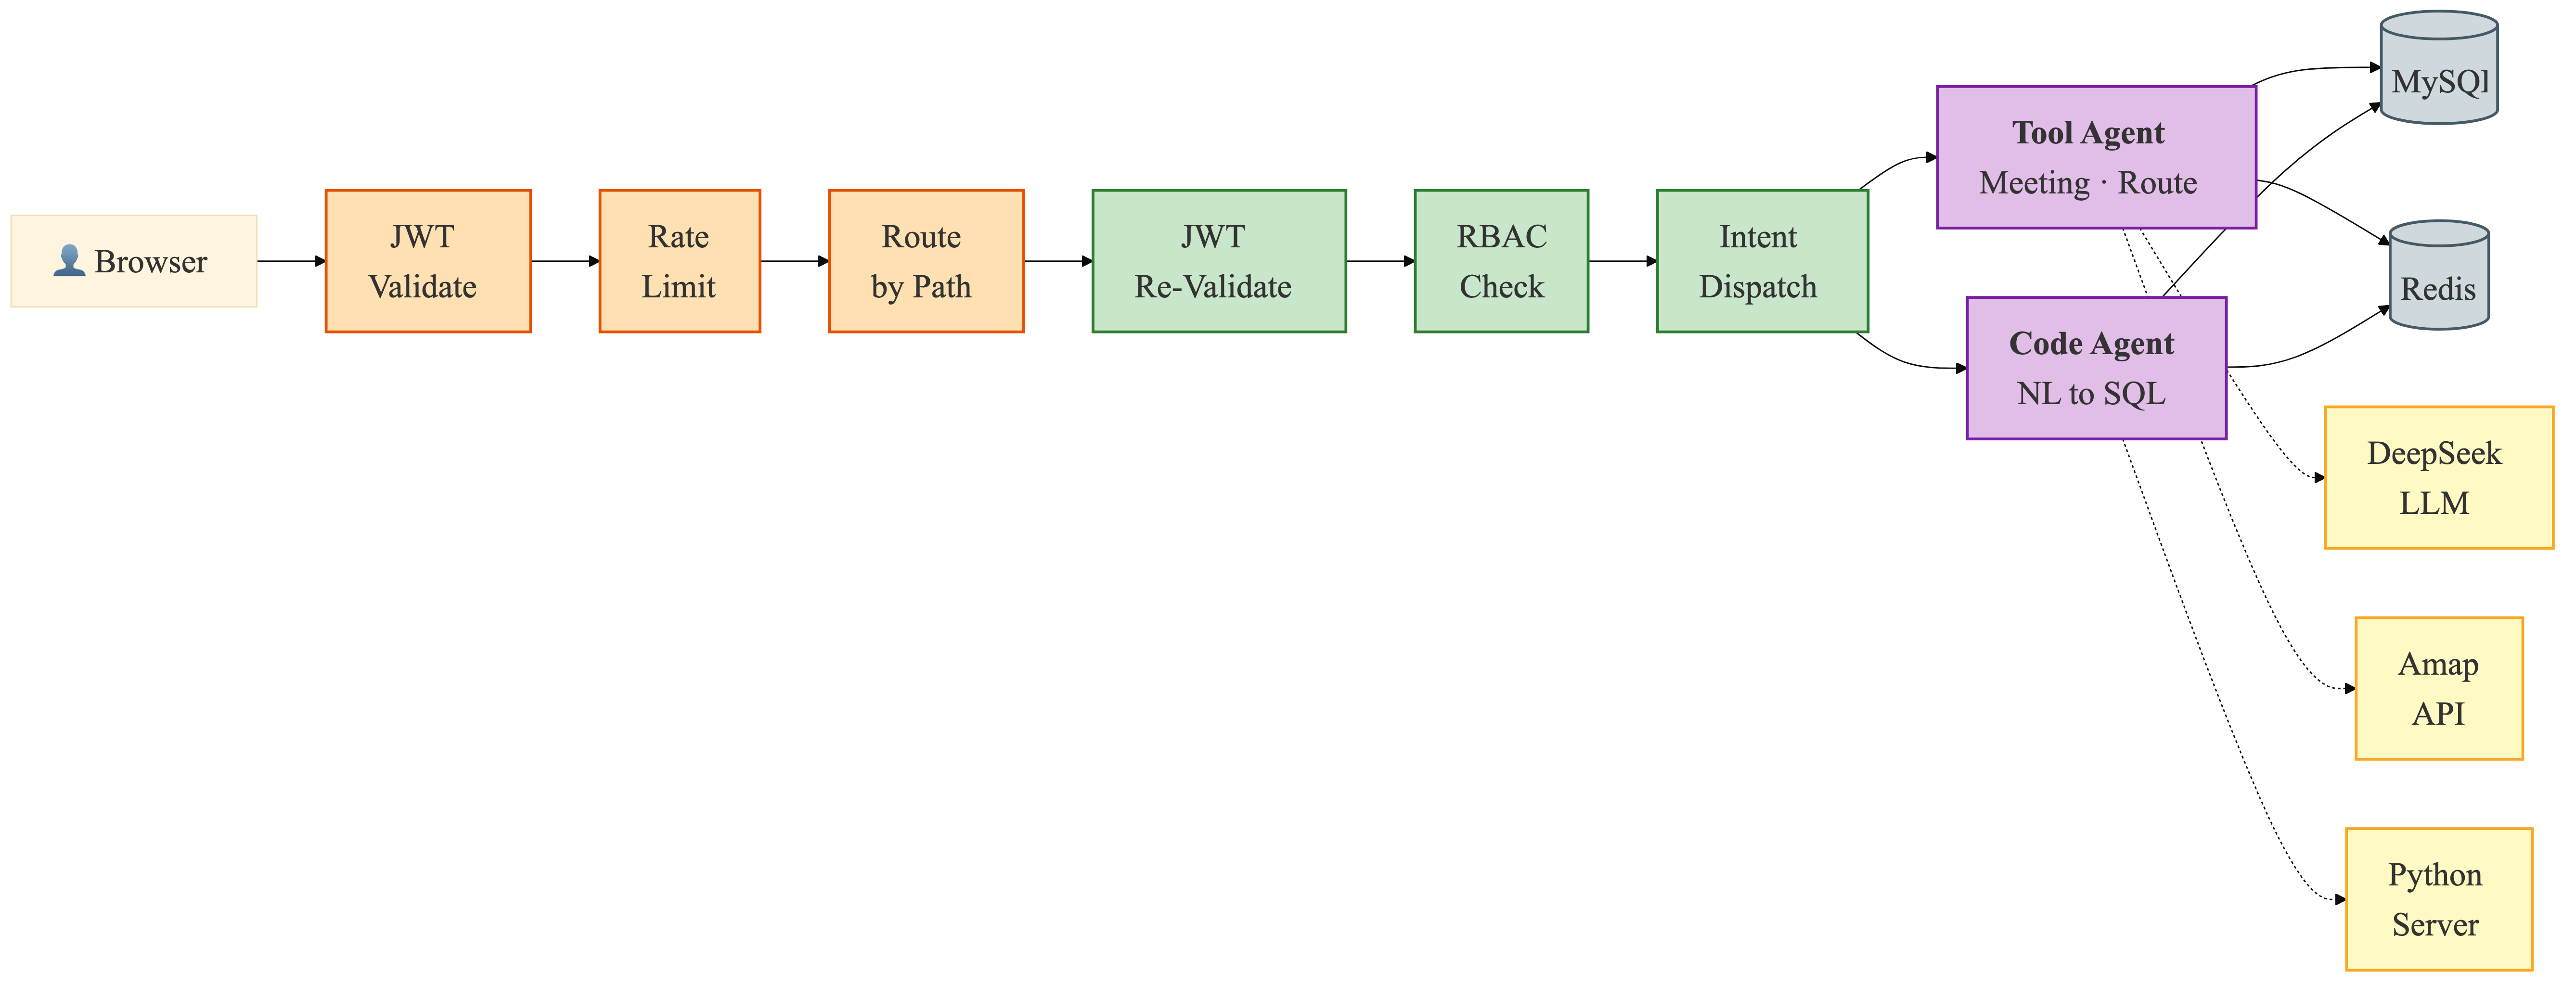
\includegraphics[width=0.92\textwidth]{figures/fig03_data_flow.png}
\caption{Data Flow Architecture --- End-to-End Request Processing Across System Layers}
\label{fig:data-flow}
\end{figure}

In the Tool agent section, the natural language query (POST /tool/execute) processing path introduces an additional semantic layer. Requests don't directly reach the business logic; instead, they are first sent to DeepSeek for intent ``translation''---the model needs to understand whether the user wants to book a meeting room, check a schedule, or plan a route. Only after the intent is clear is the request routed to the corresponding domain module. Meanwhile, the code generation path (POST /code/query) follows a completely different pipeline. The service layer delegates the task to the backend Python inference server. After the SQL is returned, it undergoes a five-layer security check before the Jdbc Template is finally allowed to execute into the database. This link is significantly longer and more likely to become a bottleneck.

The asynchronous task state synchronization mechanism differs from the conventional front-end polling mode. This platform relies on the Web Socket long connection maintained by the gateway proxy to actively push the proxy execution progress to the client, thereby achieving real-time visualization without increasing the request frequency (which will hardly generate any additional latency).

\subhead{4.2 Frontend Architecture}

This project's front-end is based on Vue 3 technology stack, and actual development utilized Composition API and TypeScript. The motivation for introducing TypeScript was straightforward: we wanted to catch type errors during compilation phase, reducing runtime exceptions caused by type mismatches. The logic reuse mechanism provided by Composition API was used simultaneously in Tool, Code, RAG interfaces, and management backend---the same set of interaction logic did not need to be implemented repeatedly, thus significantly reducing maintenance cost. We believe that terminal devices used in banking environment is quite complex (desktops, laptops, tablets, and mobile phones are all used, meaning that responsive layout is not an added feature, but a fundamental constraint that must be met.

Route management is handled uniformly by Vue Router, divided into public routes and authenticated routes based on access permissions. Navigation guards intercept requests before route switching, preventing unauthorized requests from entering protected pages. AuthLayout handles the login and registration pages, featuring a slide-in animation during page transitions. MainLayout is the main framework after authentication, with a left sidebar that supports both expanded and collapsed states. When expanded, its 230 pixels wide, and when collapsed, its only 56pixels wide, just enough to accommodate a function icon. The main framework is divided into three areas: agent services (tools, code, RAG) for regular users, a management panel accessible only to ROLE\_ADMIN, and system settings. Language switching supports Simplified Chinese, Traditional Chinese, and English(meeting the requirements of Hong Kong banks) .Unread message counts is obtained by polling the /user/notification/unread-count interface every 10 seconds and displayed as badges. The user avatar dropdown menu includes a personal information entry and a logout function.

For state management, we chose Pinia and split it into two Store based on their responsibilities. The userStore is responsible for maintaining login state. JWT tokens is persistently stored in localStorage. userInfo records user roles, permissions, departments, and security levels. External call layers interact with it through the login, logout, and getUserInfo methods. The taskStore tracks the agent task lifecycle. The Task structure includes fields for id, type (code/rag/tool), status (pending/running/completed/failed), progress (0--100), result, and createTime. Status changes are handled through addTask and updateTask.

HTTP requests are uniformly encapsulated in utils/request.ts. The Axios instance is pre-configured with basic URLs and interceptors. Server-side response are uniformly packaged into a Result structure with the fields code, msg, and data. This structure is convenient for front-end response processing. WebSocket communication is handled within utils/websocket.ts, using the wsClient singleton pattern to manage the connection lifecycle. It automatically reconnects after a connection interruption, attempting a maximum of 3 times with a 2-second interval (otherwise, interaction latency would increase. Messages are handled according to four event categories: open, message, close, and error.

Map rendering is handled by the MapContainer.vue component. This component dynamically injects the Amap JS API v2.0, carrying the API key and security code. The map expands from the starting coordinates, with the route drawn as an indigo (\#4f46e5) polyline, 6 pixel wide. Custom icons in green and red are used for the start and end points respectively (we've compared them, and color differences improve visibility). The easeOutQuad easing function is used for navigation transitions, making highlight transitions smoother. Full-screen loading feedback is implemented by AgentThinking.vue, with a Sparkles icon placed in center of the screen and a carousel displaying the thinking state text below, the content sourced from a configurable array. The progress bar uses a gradient design, and the progress value will never reach 100\% during the loading process. It will fill up instantly when the task is actually completed. This detail is to avoid the user feeling that they are ``stuck in the last little segment''.

Table \ref{tab:frontend-tech-stack} summarizes the frontend technology stack.

\vspace{3mm}

\begin{table}[H]
\small\singlespacing
\centering
\caption{Frontend Technology Stack Specifications}
\label{tab:frontend-tech-stack}
\vspace{2mm}

\begin{tabular}{@{}p{3cm}p{3.5cm}p{\dimexpr\textwidth-6.5cm-4\tabcolsep\relax}@{}}
\toprule
\textbf{Component} & \textbf{Technology} & \textbf{Utility \& Responsibility} \\
\midrule
View Layer       & Vue 3 + TypeScript            & Composition API with strict type safety \\
State Management & Pinia                         & userStore (JWT persistence), taskStore (task lifecycle) \\
UI Components    & Element-Plus                  & Enterprise forms, tables, dialogs, navigation elements \\
Visualization    & ECharts 5                     & Rendering of data charts and SQL execution result analytics \\
Build Tool       & Vite 4                        & Sub-second HMR during development, Rollup-based production bundling \\
HTTP Client      & Axios + Interceptors          & JWT auto-attach, 401 auto-logout, unified error handling \\
Real-Time        & WebSocket Client              & Singleton with auto-reconnect (3 attempts, 2s delay) \\
Inter\-nation\-al\-ization & Vue I18n            & zh-CN, zh-TW, en locales with Element Plus sync \\
Map Visualization & Amap JS API v2.0             & Dynamic SDK loading, route polyline, custom markers \\
\bottomrule
\end{tabular}
\end{table}


\subhead{4.3 Backend Microservice Architecture}

The backend consists of independent Spring Boot micro service, each handling a specific business capability and communicating through the Gateway layer. This decomposition allows independent development, testing, deployment, and scaling of each service, while the Gateway provides a single API entry point for the frontend.

Gateway Service (port 8080). Built on Spring Cloud Gateway 3.1.9, this service provides dynamic routing based on URL path predicates. The JwtAuthGlobalFilter (a GlobalFilter with order=-100)validates tokens for non-whitelist paths. It forwards identity information to downstream services through HTTP headers (X-User-Id, X-Username, X-User-Roles, X-User-Permissions, X-User-Dept-Id, X-User-Security-Level). Single-session enforcement is used. This means when someone logs in again, the old token is deleted from Redis. IP-based rate limiting is also configured: requests sent from the same IP address cannot exceed 100 per second (the burst capacity is 200, returning HTTP 429 upon exceeding). The gateway is the only container whose port is exposed to the outside; all other services are only accessible to each other through the internal Docker network.

User Service (port 8081). This is the largest backend service, covering the complete user lifecycle. Spring Security 6.x is configured with stateless session management, CSRF disabled, and a JwtAuthenticationFilter that extracts the token from the Authorization header as the primary authentication mechanism. A dual-mode login controller accepts either password or verification code credentials, with the token signer using HMAC-SHA256 (the key is injected via environment variable). BCryptPassword Encoder (strength factor 10) handles password storage and verification. Three-tier RBAC is implemented by granting role-specific permissions to an endpoint. The access model to system documents is based on a two-dimensional matrix: clearance level (1-3) and department membership. In the notification subsystem, five state flows support threaded conversations through parent\_id and thread\_id fields. The email verification subsystem uses Resend HTTP API with HTML formatted templates.

Tool Agent Service (port 8083). The most developed AI service, it implements the Tool Agent with two controller groups. The ToolController (/tool/*) exposes 11 endpoints for end-user tool operations including room queries and reservations, CRUD for personal schedules, conflict detection, route planning, and a unified /tool/execute natural language AI entry point. The MeetingRoomAdminController (/tool/admin/*) exposes CRUD endpoints for administrators---room and schedule management. The AI intent routing module integrates with DeepSeek API (via iFlytek MaaS) for intent classification, routing requests to MeetingHandler, ScheduleHandler, or RouteHandler accordingly, with MockDetectFallback providing graceful degradation when the API is unavailable.

Code Agent Service (port 8084). Implements the NL2SQL pipeline. The OnnxCodeGenerationService (enabled through the code-agent.onnx.enabled=true property) is the sole CodeGenerationService implementation, acting as an HTTP client proxy to the Python inference server. It is responsible for constructing the prompt (including database schema information), forwarding the natural language question, and extracting the generated SQL from the response. The Sql Validation Service performs five-layer whitelist checking. The MetadataCacheManager periodically refreshes the schema metadata cache from information\_schema to Redis, so the LLM always has an up-to-date view of the table structure.

Task Service (port 8082). Currently scaffolded with a basic POM configuration and TaskApplication main class. In the current architecture, task orchestration is distributed between the Gateway (request routing) and each agent service (autonomous execution). The separate task service is planned for centralizing asynchronous task tracking, progress management, and cross-agent workflow coordination in future phases.

Table \ref{tab:backend-services} summarizes the backend services.

\vspace{3mm}

\begin{table}[H]
\small\singlespacing
\centering
\caption{Backend Service Ecosystem and Technical Orchestration}
\label{tab:backend-services}
\vspace{2mm}

\begin{tabular}{@{}p{3cm}p{3.5cm}p{\dimexpr\textwidth-6.5cm-4\tabcolsep\relax}@{}}
\toprule
\textbf{Component} & \textbf{Technology} & \textbf{Utility \& Responsibility} \\
\midrule
Gateway Layer        & Spring Cloud Gateway 3.1.9  & Dynamic routing, JWT validation, IP rate limiting, WebSocket proxy \\
Business Logic       & Spring Boot 3.x + MyBatis-Plus & Service orchestration, type-safe CRUD, logical deletion (@TableLogic) \\
Security Framework   & Spring Security 6.x + JWT   & Stateless authentication, RBAC with @PreAuthorize, BCrypt password hashing \\
Caching Layer        & Spring Data Redis           & Session caching, rate limit counters, metadata cache \\
AI Integration (Tool) & DeepSeek API (HTTPS)       & Intent routing (MEETING/SCHEDULE/ROUTE), parameter extraction, route translation \\
Inference Engine     & Python FastAPI (port 8090)  & LLM-based SQL generation from natural language questions via /infer endpoint \\
RAG Agent            & Spring Boot 3.x (port 8085) & Document Q\&A, vector retrieval, source citation, access workflow \\
Embedding Worker     & Python FastAPI (rag-worker) & bge-m3 embedding generation, Markdown chunking \\
Document Parsing     & Apache Tika                 & Multi-format document parsing for RAG ingestion pipeline \\
Vector Retrieval     & Milvus Java SDK 2.3+        & Semantic ANN search for RAG document retrieval \\
Object Storage       & MinIO                       & Document file storage (PDF/DOCX/PPT), Milvus backend \\
Email Service        & Resend API                  & Email verification code delivery, three-tier rate limiting \\
Map Services         & Amap API (HTTPS)            & Geocoding (multi-level fallback), direction calculation, polyline coordinate parsing \\
\bottomrule
\end{tabular}
\end{table}

\subhead{4.4 Gateway and Security Design}

Data security is paramount in banking systems. Therefore, our platform's security design does not rely on a single line of defense, but rather incorporates defense in depth across all layers. Each layer is independently verified before a request can pass through, which make it significantly harder for a single component failure to lead to a data breach or security incident.

Figure \ref{fig:jwt-auth-flow} shows the complete user authentication flow in three stages, including the email verification code mechanism that supports both registration and code-based login.

\begin{figure}[H]
\centering
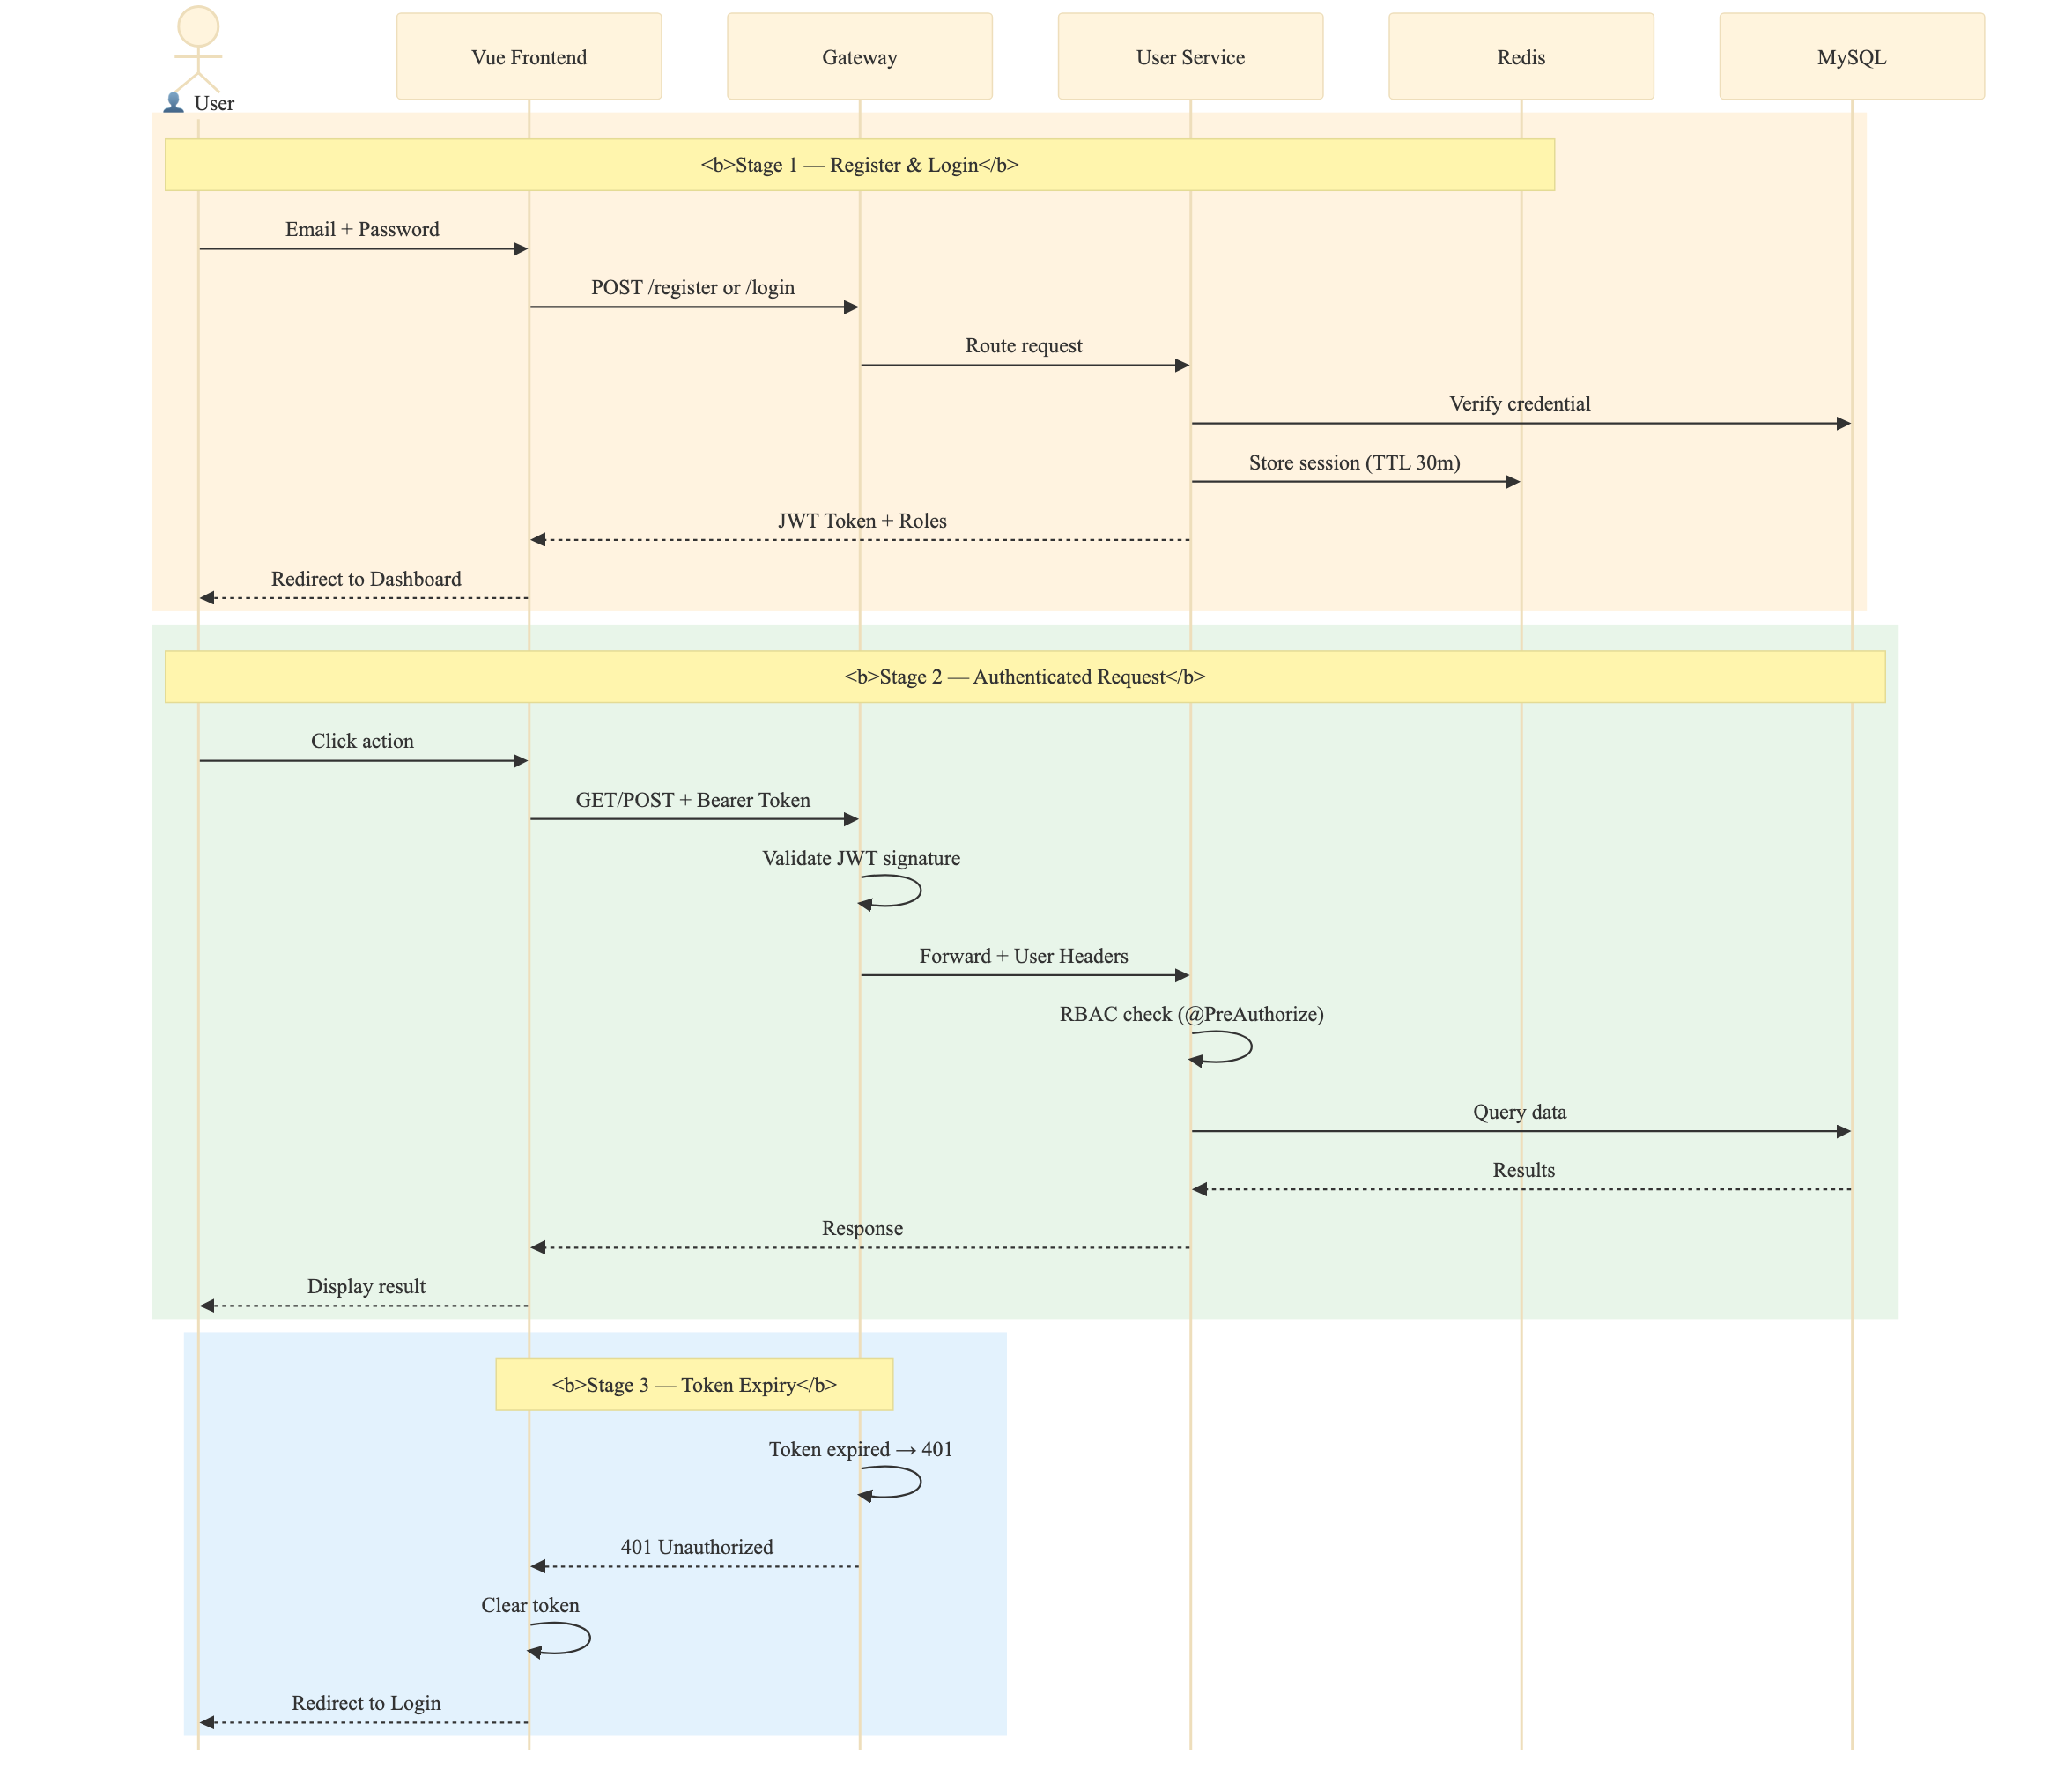
\includegraphics[width=0.92\textwidth]{figures/fig04_jwt_auth_flow.png}
\caption{JWT Authentication and Email Verification Flow}
\label{fig:jwt-auth-flow}
\end{figure}

The login process begins with an email verification code. We migrated the email delivery mechanism from QQ Mail SMTP to the \textbf{Resend HTTP API}, eliminating the connection instability and vendor-specific risk controls associated with private SMTP relays while leveraging Resend's managed infrastructure for higher deliverability and operational traceability. The HTML verification email template was redesigned to render the 6-digit code in a \textbf{monospace font}, reducing user misreading errors caused by visually similar character pairs (e.g., ``0'' versus ``O'', ``1'' versus ``l'').

After the user submits their email address on the front end, the request reaches the user service section. The service enforces a \textbf{three-tier rate-limiting strategy} backed by Redis. \textbf{Tier 1} imposes a 60-second cooldown per email address (Redis key \texttt{rate:email:send:\{email\}}), preventing rapid-fire brute-force attempts. \textbf{Tier 2} adds an IP-level hourly quota of maximum 5 requests per IP per hour, mitigating distributed enumeration attacks where the adversary rotates target addresses while sharing a common network egress; to ensure accurate IP attribution behind the gateway layer, the \texttt{UserController} extracts the real client IP from the \texttt{X-Forwarded-For} and \texttt{X-Real-IP} headers rather than using the immediate TCP connection endpoint. \textbf{Tier 3} enforces a daily ceiling of 10 requests per individual email address, preventing persistent resource exhaustion and harassment. Only after all three tiers are passed does the service call the Resend HTTP API using WebClient. The recipient email address is injected into the HTML template at the \{email\} placeholder, and the generated 6-digit random verification code is stored in Redis with a 5-minute TTL. The front-end receives a success response, triggers a 60-second countdown to disable the send button, and displays the sample email in an Alert.

These architectural changes are formally documented in \texttt{docs/email-verification-design.md}, which includes a complete system architecture diagram illustrating the end-to-end flow from client request through gateway routing, tiered rate-limiting evaluation, Resend API dispatch, and Redis state management.

Specifically, the registration process requires the user to submit their email address, verification code, and password. The backend retrieves the verification code from Redis and compares it. If successful, it creates the user record (with the password hashed by BCrypt), immediately deletes the verification code from Redis, and returns a JWT. Attempts exceeding 5 incorrect verification attempts will cause the verification code to be forcibly invalidated and the user need to request a new one. For the multi-level rate limiting, the code brute-force crack protection is covered in NFR3.

In subsequent requests, the frontend automatically appends a Bearer Token via an Axios interceptor. the gateway layer's JwtAuthGlobalFilter is responsible for signature verification, checking the validity period and extracting the payload. The whole process is statless---the backend does not keep session state---so the system can be scaled horizontally seamlessly. This approach avoids the common performance and availability issues associated with centralized session storage.

The CAPTCHA itself is also heavily reinforced: the 6-digit random number only lasts for 5 minutes and is immediately deleted from Redis after successful verification, ensuring single-use semantics; a maximum of 5 incorrect attempts trigger forced invalidation; the 60-seconds cooldown effectively prevents SMS bombing attacks, so the CAPTCHA security is not something we overlooked.

We adopted RBAC for our permission design, but only implemented a coarse-grained division of roles into three tiers---this ``coarseness'' was intentional. Different banks have vastly different organizational structures and reporting relationships; fine-tuning the details ourselves would inevitably not match a real deployment scenario. So, we chose to provide a clear foundational role framework and leave the detailed permission customization to the bank's own IT administrators.

\begin{table}[H]
\small\singlespacing
\centering
\caption{Pseudocode --- listDocumentsForUser() Multi-Factor Document Access Rule}
\label{tab:pseudocode-list-docs}
\vspace{2mm}

\begin{lstlisting}
FUNCTION listDocumentsForUser(userId, userDeptId, userClearance)
    documents = queryAllDocuments()
    result = []
    FOR EACH doc IN documents:
        // Multi-factor access rule: a document is visible if...
        IF doc.dept_id IS NULL THEN
            // Global document - accessible to all users
            doc.accessible = TRUE
        ELSE IF doc.dept_id = userDeptId
                 AND doc.security_level <= userClearance THEN
            // Same department with sufficient clearance
            doc.accessible = TRUE
        ELSE
            // Access denied - user may submit escalation request
            doc.accessible = FALSE
            doc.escalationType = "RAG_APPLY"
            // Manager can approve (Pending -> Approved) or deny (Pending -> Denied)
        END IF
        result.add(doc)
    END FOR
    RETURN result
END FUNCTION
\end{lstlisting}
\end{table}


The unified exit point for external communication is the REST API, all using HTTPS, with the TLS version locked at 1.3. WebSocket is forcibly upgraded to WSS in the production environment; this switch is handled in the code by checking the protocol in the Nginx X-Forwarded-Proto header, with the backend redirecting HTTP traffic to HTTPS.

\subhead{4.5 Data Layer Architecture}

For the data persistence layer, we adopted a multi-engine heterogeneous architecture. The main reason for not using a single database were the significant difference in storage requirements for different data types---storing vectors, relational data, and cache data all in MySQL would have created performance bottlenecks and architectural complexity. Instead, three specialized storage engines were deployed, each optimized for its specific data type.

All relational data resides on MySQL 8.0. We agreed on the database name agent\_platform, character set utf8mb4, and collation utf8mb4\_unicode\_ci---while general\_ci is more faster, it causes garbled characters in Chinese and emoji symbols. This design is essential for internationalization (including Traditional Chinese). The complete schema (9 tables) and seed data are documented in Appendix A.

The user and permission management uses five tables: sys\_user stores account information, passwords are hashed using BCrypt, and it's linked to sys\_department as foreign key, also recording security levels (1-3). sys\_role defines three role codes (ROLE\_ADMIN, ROLE\_DEPT\_ADMIN, ROLE\_USER). sys\_permission defines six granular permissions covering user management, role management, and department management. sys\_user\_role is a many-to-many association table connecting users to roles, and sys\_role\_permission connects roles to granular permissions. The primary identity management process relies on the RBAC model described in the security section. For document management, the sys\_document table stores knowledge base content with clearance levels and department associations. Meeting room management uses meeting\_room and meeting\_schedule tables, where schedule records include room\_id FK, booker, start\_time, end\_time, and attendee list.

During system initialization, we added a batch of seed data: four meeting rooms, five users with different roles and security levels, six departments, six permissions, a complete role allocation relationship tree, and eleven system documents covering banking compliance scenarios.

Cache and high-frequency operational data are handled by Redis 5.0+. Session tokens are stored in memory with configurable TTLs; atomic counting also rely on Redis when the gateway layer performs IP-level rate limiting (INCR + EXPIRE is the only strategy we use, it's simple, reliable, and effectively prevents race conditions). The JWT single-session mechanism is implemented through Redis keys token:username: \{username\}; on each login, the system invalidates any existing token for the same user.

Redis is also used for the tool's intelligent agent's schedule conflict detection. The key format is tool:schedule:\{userId\}. We store the meeting timestamps as scores using an ordered set. For overlapping queries, we use ZRANGEBYSCORE to retrieve entries whose startEpoch is within the query time window. The operation has logarithmic time complexity for both insertion and query. For MySQL-Redis consistency, we adopted a scheme of ``write MySQL first, then write Redis, and delete the Redis key on failure,'' this is basically a simple cache-aside pattern, prioritizing strong consistency for persistent data.

Semantic retrieval for RAG agents requires vector support, so we separately introduced Milvus 2.3+. During the selection process, we considered several vector engines, and Milvus, with its relatively advanced four-tier architecture (access layer, coordinator, worker node, and object storage), ultimately stood out for enterprise deployment scenarios. Milvus's collection schema is dynamically configured at startup, with dimension matching the embedding model dimension (default 4096), metric type set to IP (inner product), and index type supporting IVF\_FLAT and HNSW.

Going forward, we plan to add a security post-filter to the RAG retrieval pipeline. The raw vector results returned by Milvus will not be directly passed through; instead, they will be secondarily filtered against the allowed document list computed during the pre-retrieval phase, guaranteeing enforcement even if the filter expression in the Milvus query itself fails.

Table \ref{tab:data-storage} summarizes the data storage strategy.

\vspace{3mm}

\begin{table}[H]
\small\singlespacing
\centering
\caption{Multi-Modal Data Storage Strategy and Layered Access Patterns}
\label{tab:data-storage}
\vspace{2mm}

\begin{tabular}{@{}p{2.5cm}p{2.5cm}p{5.5cm}p{\dimexpr\textwidth-10.5cm-6\tabcolsep\relax}@{}}
\toprule
\textbf{Category} & \textbf{Engine} & \textbf{Primary Data Types} & \textbf{Access Pattern} \\
\midrule
Operational Layer & MySQL 8.0   & Users, roles, departments, documents, meeting rooms, schedules, notifications & Transactional, ACID-compliant read/write \\
Caching Layer     & Redis 5.0+  & Session tokens, rate limit counters, metadata cache (hash), schedule conflicts (sorted sets) & High-concurrency, sub-millisecond reads \\
Object Storage    & MinIO       & PDF, DOCX, PPT files; Milvus backend objects & Document upload/download, RAG source document storage \\
Vector Layer      & Milvus 2.3+ & Document chunk embeddings (bge-small-zh), source metadata & Semantic approximate nearest neighbor search \\
\bottomrule
\end{tabular}
\end{table}


\subhead{4.6 Technology Stack Rationale}

After discussion, the technology stack of our system was determined based on four main principles: First, it should be able to be deployed locally to reduce reliance on external cloud services (because banking regulations require data to be stored on local servers); second, all components should work well with container technology (because we wanted the developer environment and the production environment to be as similar as possible); third, the technology stack should match the team's current skill set (backend students are more familiar with Java than Python, so AI services had a separate Python module for LLM inference tasks); fourth, we preferred ecosystems that have long-term support and active communities (so we can find an answer on Stack Overflow when hitting a problem).

Specifically, the system's backend framework uses Java + Spring Boot. This choice was primarily based on its mature enterprise-level ecosystem. A strong typing system effectively reduces implicit errors caused by type mismatches; Spring Security provides fine-grained method-level permission control support for RBAC. Each microservice is configured with an independent spring-boot-starter-parent, managed hierarchically through parent POMs to unify dependency versions.

Our gateway is Spring Cloud Gateway, rather than a traditional Servlet solution. (One issue with Servlets is that containers default to a blocking ``one thread, one request'' model. As the gateway acts as the hub for all service traffic, the extra thread overhead would have been substantial under high load. The reactive model is more suitable for the gateway's role as a proxy and filter, given its high-concurrency scenario. The gateway performs identity verification through a custom JwtAuthGlobalFilter, repackaging the token payload (user ID, roles, and permissions) into the request headers, unifing the previously scattered authentication logic.

The AI inference service ultimately chose Python + FastAPI, deployed on port 8090. Python's dominant position in the machine learning toolchain is unlikely to be replaced in the short term (compared to alternatives like Scala or R, its library ecosystem is dramatically richer). FastAPI offers performance close to Node.js while automatically generating Swagger documentation, which reduces the cost of inter-team interface coordination.

We settled on Vue 3 with TypeScript after weighing several options. While the team's front-end skill levels were uneven, Vue 3's learning curve proved less steep than alternatives, which mattered give our project schedule. TypeScript was not optional---it stopped numerous type errors at compile time that JavaScript would have silently let through. The Composition API gave us logic reuse that we actually used across all the pages that call agents that share the same skeleton of request \textrightarrow{} progress \textrightarrow{} result display logic, while the Options API would have forced code duplication.

Containerization via Docker and Docker Compose was our choice for environment parity. MySQL, Redis, and Milvus all run as containers, which eliminates the ``it works on my machine'' problem. The Java services are each packaged as thin JARs, with dependencies separated from the application code to reduce image rebuild time during iteration.

\newpage

% ======================================================================
